\begin{figure}[htbp]
\centering
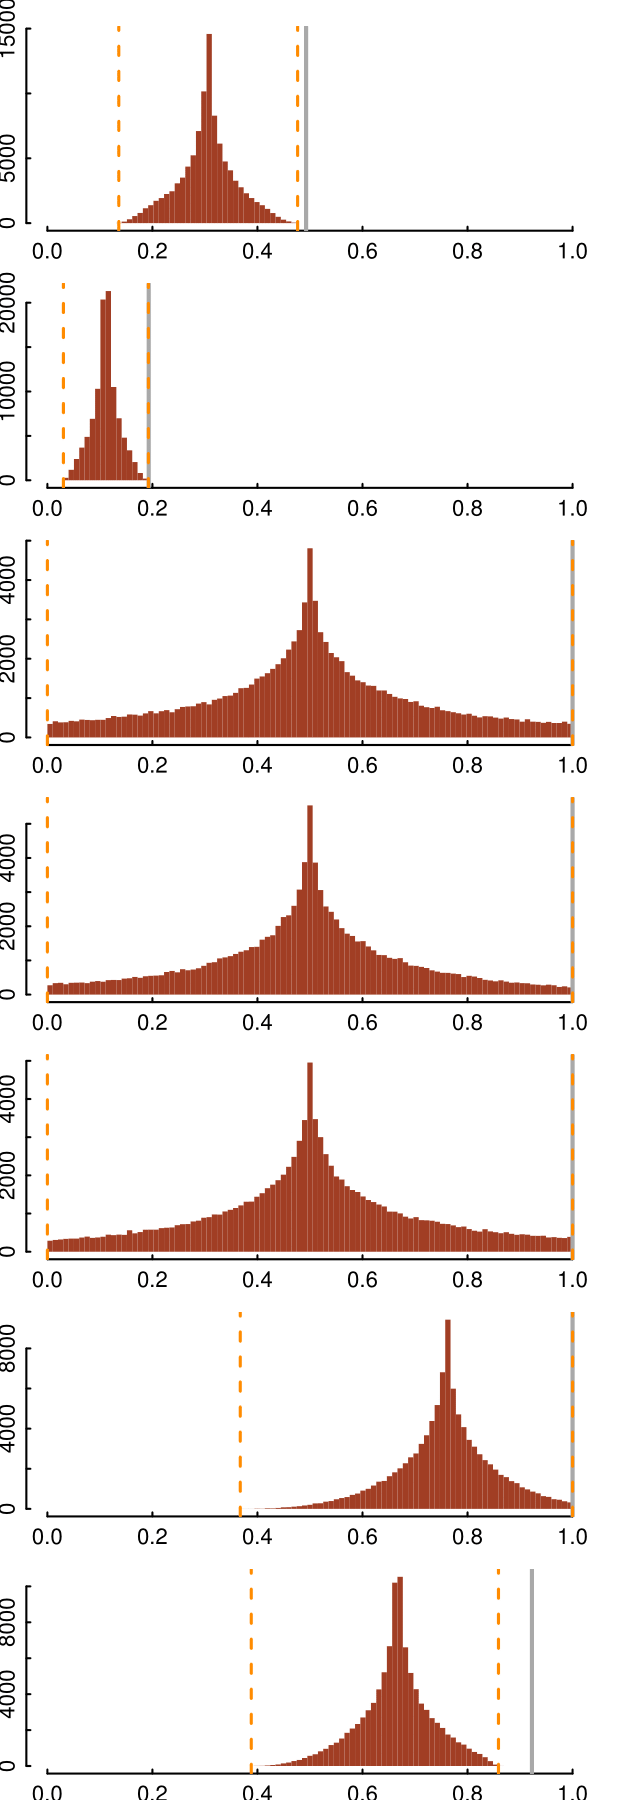
\includegraphics[width=7.5cmh]{sections/figs/raw_histograms.png}
\caption{We show one histogram for each muscle of the index finger to illustrate how the muscle is used across all feasible solutions.
For this set of distributions, the task was 50\% of maximal force output in the palmar direction. Muscles are FDP, FDS, EIP, EDC, LUM, DI, and PI are shown in that order. The orange dotted lines are the lower and upper bounds of activation.}
\label{fig:raw_histograms}
\end{figure}


\section{RESULTS}

Figure \ref{fig:raw_histograms} shows the distributions of activations resulting from $1,000,000$ solutions computed with Hit-and-Run sampling. This is the first time (to our knowledge) that the internal structure of the feasible activation set has been visualized for a sub-maximal force.

Notice that the lower and upper bounds of the activations (i.e., the dashed lines indicating their bounding box), are unhelpful in determining the actual density distribution of feasible activations.
The activation needed for the maximal force output (thick gray line) is very often not the mode of the activations at 50\% of output. It's important to note that these histograms are unidimensional- they do not illustrate the between-muscle associations.

